%%%
%%%  Template to prepare a defense of Bc./Mgr./... thesis
%%%  to be presented at MFF
%%%  (unofficial)
%%%
%%%  AUTHOR:  Arnošt Komárek
%%%           Department of Probability and Mathematical Statistics
%%%           Faculty of Mathematics and Physics, Charles University in Prague
%%%
%%%  LOG:    20150505  created by modification of some previous personal presentations
%%%          20170522  update related to new MFF logo
%%%  
%%%  ===========================================================================
\documentclass[c, 10pt]{beamer}


%%%%% Package needed if some accented letters in the presentation
%%%%% -------------------------------------------------------------
\usepackage[utf8]{inputenc}


%%%%% Most beamer settings and other LaTeX commands
%%%%% are provided in the file below
%%%%% -----------------------------------------------------
%%%
%%%  Style for MFF related presentations
%%%  (unofficial)
%%%
%%%  AUTHOR:  Arnošt Komárek
%%%           Department of Probability and Mathematical Statistics
%%%           Faculty of Mathematics and Physics, Charles University in Prague
%%%
%%%  LOG:    20150430  created by modification of some previous personal presentations
%%%          20170522  modified (new MFF logo)
%%%  
%%%  ===========================================================================

%%%%% If to determine whether Czech or English version
%%%%% of a presentation is to be produced
%%%%% default = Czech
%%%%% ------------------------------------------------------
\newif\ifCZversion
\CZversiontrue

\ifCZversion\else\renewcommand{\uv}[1]{``#1''}\fi


%%%%% Included packages
%%%%% ----------------------------------------------------------
\usepackage{helvet}                       % font
\usepackage{amsmath, amssymb}
\usepackage{delarray}
\usepackage{multicol}
\usepackage{graphicx, fancybox}
\usepackage{psfrag}
\usepackage{fancyvrb}
\usepackage{eurosym}
\usepackage{bbding}
%\usepackage{marvosym}
\usepackage{wasysym}
\usepackage[czech]{babel}

\usepackage[pdftex]{bookmark}


%%%%% Some LaTeX commands
%%%%% ----------------------------------------------------------
\renewcommand{\arraystretch}{1.2}


%%%%% Some colors and related commands
%%%%% ----------------------------------------------------------

  %% Pantone 186 = "official" red of MFF
\definecolor{redmff}{rgb}{0.7892720,0.0651341,0.1455939}          

  %% First level color = black
\definecolor{colOne}{rgb}{0,0,0}
\newcommand{\tOne}[1]{\textcolor{colOne}{#1}}
\newcommand{\tOneb}[1]{\textcolor{colOne}{\textbf{#1}}}
\newcommand{\tOnei}[1]{\textcolor{colOne}{\textit{#1}}}

  %% Second level color = quite dark blue
\definecolor{colTwo}{rgb}{0,0,0.3}                
\newcommand{\tTwo}[1]{\textcolor{colTwo}{#1}}
\newcommand{\tTwob}[1]{\textcolor{colTwo}{\textbf{#1}}}
\newcommand{\tTwoi}[1]{\textcolor{colTwo}{\textit{#1}}}

  %% Third level color = something between blue3 and blue4
\definecolor{colThree}{rgb}{0,0,0.7}              
\newcommand{\tThree}[1]{\textcolor{colThree}{#1}}
\newcommand{\tThreeb}[1]{\textcolor{colThree}{\textbf{#1}}}
\newcommand{\tThreei}[1]{\textcolor{colThree}{\textit{#1}}}

  %% Color to alert (highlight) = MFF red
\definecolor{alertCol}{rgb}{0.7892720,0.0651341,0.1455939}
\newcommand{\tal}[1]{\alert{#1}}
\newcommand{\talb}[1]{\textbf{\alert{#1}}}
\newcommand{\tali}[1]{\textit{\alert{#1}}}

  %% White
\newcommand{\tw}[1]{\textcolor{white}{#1}}
\newcommand{\twb}[1]{\textcolor{white}{\textbf{#1}}}
\newcommand{\twi}[1]{\textcolor{white}{\textit{#1}}}

  %% Some other colors used somewhere
\definecolor{semiwhite}{gray}{0.98}
\definecolor{mffgray}{gray}{0.95}
\definecolor{semiblack}{gray}{0.5}
\definecolor{rred}{rgb}{0.5,0,0}


%%%%% Beamer stuff
%%%%% ----------------------------------------------------------
\mode<presentation> {

    %%% General theme of a presentation (some pre-specified themes)
    %%% ------------------------------------------------------------------
    %\usetheme{CambridgeUS}
    \usetheme{Warsaw}

    %%% Color schemes that will be used unless redefined below
    %%% ------------------------------------------------------------------
    %\usecolortheme{wolverine}
    \usecolortheme{beaver}


    %%% Color schemes for different elements of a presentation
    %%% ---------------------------------------------------------

      %%% Uncomment the two rows below if some background file (layout) is to be used
      %%% on all slides
    %\usebackgroundtemplate{
\includegraphics[width=\paperwidth, height=\paperheight]{./FigureLayout/BackgroundRotunda}}
    %\setbeamercolor{background canvas}{bg=}                                                             

      %%% Setting for "standard" slides
      %%% - must be commented if background file used
    \setbeamertemplate{background canvas}[vertical shading][bottom=semiwhite, top=white, middle=semiwhite!50!white]
    \setbeamercolor{background canvas}{bg=white}                           %% NO EFFECT WHEN \setbeamertemplate{background canvas} WAS USED

      %%% Colors of frametitle, normal, alerted and math texts
    \setbeamercolor{frametitle}{fg=white, bg=redmff}
    \setbeamercolor{normal text}{fg=black}
    \setbeamercolor{alerted text}{fg=redmff}
    \setbeamercolor{math text inlined}{fg=colTwo}
    \setbeamercolor{math text displayed}{fg=colTwo}

      %%% Colors for some special boxes defined below
    \setbeamercolor{mffboxcol}{fg=colTwo, bg=mffgray}
    \setbeamercolor{mffboxcolupper}{fg=white, bg=redmff}

    %%% Set serif font (patkové písmo) in mathematics
    %%% ------------------------------------------------
    %\usefonttheme[onlymath]{serif}

    %%% Itemize style (rectangles instead of bullets)
    %%% ------------------------------------------------
    %\useinnertheme{rectangles}

    %%% Default content of a header of each slide
    %%% (currently nothing)
    %%% ------------------------------------------------
    \setbeamertemplate{headline}{}

    %%% Default content of a foot of each slide
    %%% ------------------------------------------------
    %\setbeamercolor{page number in head/foot}{fg=black, bg=white}
    \setbeamertemplate{footline}{
      \hspace*{2.5em}
      \begin{beamercolorbox}{section in head/foot}
      \vskip1pt
      \tOne{\rule{\textwidth}{1pt}}
      \vskip2pt

      %%% Foot containing (a) page number/total number of pages, (b) name, (c) short title of presentation
      {\small \tOne{\insertframenumber}\textcolor{semiblack}{/\inserttotalframenumber}}\hspace{1em}
      \tOne{\footnotesize \insertauthor}\hfill
      \textcolor{redmff}{\footnotesize\insertshorttitle\hspace{3em}}

      %%% Foot containing (a) page number/total number of pages, (b) name, (c) short section title
      %{\small \tOne{\insertframenumber}\textcolor{semiblack}{/\inserttotalframenumber}}\hspace{1em}
      %\tOne{\footnotesize \insertauthor}\hfill
      %\textcolor{redmff}{\footnotesize\thesection. \insertsection\hspace{3em}}
    
      \hspace*{3.5em}
      \vskip3pt
      \end{beamercolorbox}
    }

    %%% Title page
    %%% -------------------
    \setbeamertemplate{title page}{
      %\vspace*{-0.5em}
      \begin{center}
      \textcolor{black}{\normalsize\bfseries\rmfamily \insertinstitute}

      \vspace{1em}
        
      \ifCZversion
        
\includegraphics[width=0.8\textwidth]{./FigureLayout/mff_cz_color}
      \else
        
\includegraphics[width=0.8\textwidth]{./FigureLayout/mff_en_color}
      \fi

      \medskip
      \noindent\textcolor{redmff}{\rule{\textwidth}{2pt}}
  
      \bigskip
      \textcolor{black}{\normalsize\bfseries \insertauthor} \\[0.5ex]

      \bigskip
      \textcolor{redmff}{\Large\bfseries \inserttitle}

      \medskip
      \textcolor{redmff}{\large\insertsubtitle}

      \medskip
      \noindent\textcolor{redmff}{\rule{\textwidth}{2pt}}
      
      \medskip
      \textcolor{colTwo}{\small \insertdate}
      \end{center}
    }    

    %%% Switch-off/on foot with navigation symbols    
    %%% -----------------------------------------------
    % \setbeamertemplate{navigation symbols}{}
    \usenavigationsymbolstemplate{}

    %%% Left and right margin
    %%% --------------------------------
    %\setbeamersize{text margin left=1cm}
    %\setbeamersize{text margin right=1cm}


    %%% Use of a logo on each slide
    %%% (not really recommended, so commented)
    %\logo{
\includegraphics[height=1.5cm, width=1.5cm]{./FigureLayout/mff_logo}}
}


%%%%% Commands to produce slides at the beginning of each section
%%%%% --------------------------------------------------------------
\renewcommand{\thesection}{\arabic{section}}
\newcommand{\framesection}{
  \begin{frame}%[plain]

  \vspace*{2em}
  \begin{center}\Large
  \ifCZversion Oddíl \thesection \else Section \thesection \fi
  \end{center}

  \begin{center}\color{rred}\Large
  \insertsection
  \end{center}

  \end{frame}
}


%%%%% Style for software related stuff
%%%%% ----------------------------------------------------------
\newcommand{\Rko}{
\includegraphics[width=5.094mm, height=3.876mm]{./FigureLayout/Rlogo}}
\newcommand{\Rfun}[1]{\textcolor{redmff}{\texttt{#1}}}

\DefineVerbatimEnvironment{Rin}{Verbatim}{formatcom=\color{redmff}, fontsize=\scriptsize, frame=single, framerule=1pt, framesep=2pt}
\DefineVerbatimEnvironment{Rout}{Verbatim}{formatcom=\color{blue}, fontsize=\scriptsize, frame=single, framerule=1pt, framesep=2pt}


%%%%% Boxes
%%%%% ----------------------------------------------------------
\newcommand{\mffbox}[2][0pt]{%
  \begin{beamercolorbox}[center, sep=#1, rounded=true, shadow=true]{mffboxcol}
  #2
  \end{beamercolorbox}
}

\newcommand{\mffboxTitle}[2]{%
  \begin{beamerboxesrounded}[lower=mffboxcol, upper=mffboxcolupper, shadow=true]{#1}
  #2
  \end{beamerboxesrounded}
}


%%%%% Some constructions for displayed math
%%%%% ----------------------------------------------------------
\newcommand{\dmath}[2][-1.4em]{%
  \begin{beamercolorbox}[center, sep=#1, rounded=true, shadow=true]{mffboxcol}
  \begin{displaymath}
  #2
  \end{displaymath}
  \end{beamercolorbox}
}

\newcommand{\dalign}[2][-1.4em]{%
  \begin{beamercolorbox}[center, sep=#1, rounded=true, shadow=true]{mffboxcol}
  \begin{align*}
  #2
  \end{align*}
  \end{beamercolorbox}
}

\newcommand{\dgather}[2][-1.4em]{%
  \begin{beamercolorbox}[center, sep=#1, rounded=true, shadow=true]{mffboxcol}
  \begin{gather*}
  #2
  \end{gather*}
  \end{beamercolorbox}
}



%%%%% \ifCZversion is defined inside MFF_Present.sty
%%%%% to distinguish between Czech and English presentations
%%%%% ------------------------------------------------------
\CZversiontrue       %% for presentations in Czech (Slovak)
%\CZversionfalse      %% for presentations in English


%%%%% Uncomment appropriate choice below if you wish to create
%%%%% notes for audience having 2 or 4 slides on each (A4) page.
%%%%% -------------------------------------------------------------
\usepackage{pgfpages}
%\pgfpagesuselayout{4 on 1}[a4paper, landscape, border shrink=5mm]
%\pgfpagesuselayout{2 on 1}[a4paper, border shrink=5mm]

\graphicspath{ {FigureLayout/} }  % path to images folder

\usepackage{dcolumn}        % improved alignment of table columns
\usepackage{booktabs}       % improved horizontal lines in tables


%%%%% Basic settings of the document
%%%%% (will be automatically used to create a title page, foots etc.)
%%%%% --------------------------------------------------------------------

  %%% Main title
  %%% - short and long version
  %%%   --> will appear on place where \inserttitle and \insertshorttitle commands used
  %%%   --> if the full title is short enough, both short and long versions might be the same
\title[Board game with artificial intelligence]{%                       
       Board game with artificial intelligence}

  %%% Subtitle (comment it if you do not want to have it)
  %%%   --> will appear on place where \insertsubtitle and \insertshortsubtitle commands used
\subtitle[]{Obhajoba bakalářské práce}

  %%% Author
  %%% - as "short" version, link to the author's webpage is used
  %%%   (e.g., e-mail is also a useful alternative)
  %%%   --> will appear on places where \insertauthor and \insertshortauthor commands used
\author[daniel.crha(at)gmail.com]{%
        Daniel Crha}

  %%% Author's affiliation
  %%% - can be fully commented for defense presentation
  %%%   --> will appear on places where \insertinstitute and \insertshortinstitute commands used
\institute[KTIML]{%
           Katedra teoretické informatiky a~matematické logiky}

  %%% Date of presentation
  %%% - replace it by real date in case of a defense presentation
  %%%   --> will appear on places where \insertdate and \insertshortdate commands used
\date[7.7.2020]{%
      7. července 2020}


\begin{document}

%%%%% Title slide
%%%%% =====================================================================================
\frame[plain]{\titlepage}


%%%%% Fictitious introductory section
%%%%% =====================================================================================
\section{Úvod}
%\framesection{}     %%% Uncomment it to get a special slide with the section title
                     %%% - not really needed for a presentation lasting 10 minutes


  %%%%% Slide
  % ----------------------------------------------------------------------------------------
\begin{frame}\frametitle{Úvod}
\framesubtitle{Problematika}

    \begin{itemize}\itemsep=1em
    \item Klasické problémy teorie her jsou dobře prozkoumané
        \begin{itemize}\color{colTwo}\itemsep=1ex
            \item Mají i dobrou podporu
        \end{itemize}
    \item Tyto problémy ale často nemodelují reálný svět
    \end{itemize}
\end{frame}


  %%%%% Slide
  % ----------------------------------------------------------------------------------------
\begin{frame}\frametitle{Úvod}
    \framesubtitle{Složitější vlastnosti v teorii her}

    \begin{itemize}\itemsep=1em
    \item Chtěli bychom zkoumat vlastnosti, které reálný svět modelují
    \item Konkrétně:
        \begin{itemize}\color{colTwo}\itemsep=1ex
            \item Neúplnost informace
            \item Více hráčů
            \item Prvky náhody
            \item Netriviální větvící faktor
        \end{itemize}
    \item Jedná se o méně zkoumanou oblast
    \end{itemize}
\end{frame}

  %%%%% Slide
  % ----------------------------------------------------------------------------------------
\begin{frame}\frametitle{Cíle}
\framesubtitle{}

    \begin{itemize}\itemsep=1em
        \item Navrhnout hru se zmíněnými vlastnostmi
        \item Hru implementovat s~podporou pro umělou inteligenci
        \item Implementovat a~porovnat několik inteligencí
    \end{itemize}
\end{frame}

  %%%%% Slide
  % ----------------------------------------------------------------------------------------
\begin{frame}\frametitle{Návrh hry}
\framesubtitle{Pravidla a vlastnosti}
    
    \begin{itemize}\itemsep=1em
        \item Hra se jmenuje \alert{Colonizers}
        \item 4 hráči
        \item Hra se hraje v kolech s~fázemi
    \end{itemize}
\end{frame}

  %%%%% Slide
  % ----------------------------------------------------------------------------------------
\begin{frame}\frametitle{Návrh hry}
\framesubtitle{Pravidla a vlastnosti}
    \begin{figure}[ht]
        \centerline{\mbox{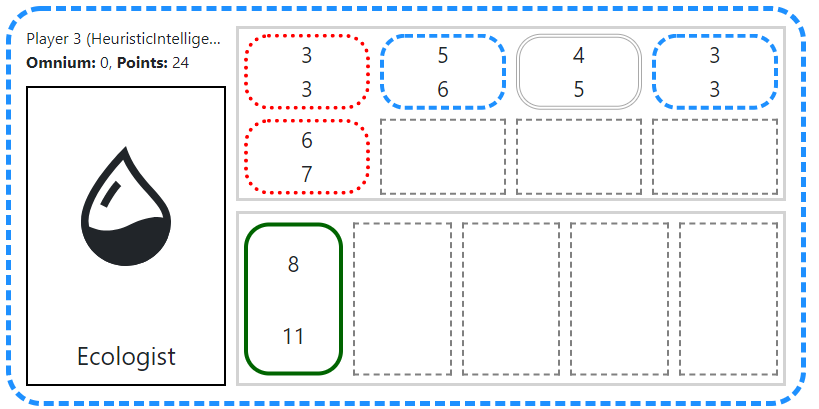
\includegraphics[width=110mm]{player}}}
        \caption{Přehled hráče.}\label{ud:player}
    \end{figure}
\end{frame}

  %%%%% Slide
  % ----------------------------------------------------------------------------------------
\begin{frame}\frametitle{Implementace}
\framesubtitle{Technologie}
    \begin{itemize}\itemsep=1em
        \item GUI - Electron + Angular
        \item Logika - C\# (.NET Core)
            \begin{itemize}\color{colTwo}\itemsep=1ex
                \item ASP.NET Core jako backend pro GUI
            \end{itemize}
        \item Umělé inteligence - Python
    \end{itemize}
\end{frame}

  %%%%% Slide
  % ----------------------------------------------------------------------------------------
\begin{frame}\frametitle{Implementace}
\framesubtitle{Rozhraní pro umělou inteligenci}
    \begin{itemize}\itemsep=1ex
        \item Inteligence implementuje bázovou třídu
        \begin{itemize}\color{colTwo}\itemsep=1ex
            \item Na ní implementuje callback
        \end{itemize}
        \item Bázová třída má další funkcionality
        \begin{itemize}\color{colTwo}\itemsep=1ex
            \item Determinizace
            \item Simulace
        \end{itemize}
        \item Soubor s umělou inteligencí je spouštěn jako \alert{\_\_main\_\_}
    \end{itemize}
\end{frame}

  %%%%% Slide
  % ----------------------------------------------------------------------------------------
\begin{frame}\frametitle{Umělé inteligence}
\framesubtitle{Implementované typy}
    \begin{itemize}\itemsep=1ex
        \item Náhodná inteligence
        \item Heuristická inteligence
        \item MaxN
            \begin{itemize}\color{colTwo}\itemsep=1ex
                \item Rozšíření Minimaxu na hry s více hráči
                \item Determinizace + poziční vyhodnocování
            \end{itemize}
        \item ISMCTS
            \begin{itemize}\color{colTwo}\itemsep=1ex
                \item Monte Carlo metoda
                \item Determinizace + simulace
            \end{itemize}
    \end{itemize}
\end{frame}

  %%%%% Slide
  % ----------------------------------------------------------------------------------------
\begin{frame}\frametitle{Experimenty}
\framesubtitle{Vybalancování hry}
    \begin{table}[h!]
        \centering
        \begin{tabular}{l@{\hspace{1.5cm}} c c c c}
        \textbf{Pozice} & \textbf{1} & \textbf{2} & \textbf{3} & \textbf{4} \\
        \midrule
        Výhry            & 230 & 202   & 282   & 286 \\
        Prohry          & 415 & 298   & 152   & 135 \\
        Průměrný výsledek    & 2.8 & 2.67 & 2.302 & 2.228 \\
        \bottomrule
        \end{tabular}
        \caption{Výsledky hraní heuristických inteligencí, 1000 her.}\label{tabex:heuristicwins}
    \end{table}
\end{frame}

  %%%%% Slide
  % ----------------------------------------------------------------------------------------
\begin{frame}\frametitle{Experimenty}
\framesubtitle{Vybalancování hry}
    \begin{itemize}
        \item $\chi^{2}$ test pro binomické rozdělení
        \item Odchylka proher na 1. a 4. místě je statisticky významná
    \end{itemize}
\end{frame}

  %%%%% Slide
  % ----------------------------------------------------------------------------------------
\begin{frame}\frametitle{Experimenty}
\framesubtitle{Porovnání inteligencí}
    \begin{table}[h!]
        \centering
        \begin{tabular}{l@{\hspace{1.5cm}} c c c c}
        \textbf{AI} & \textbf{Random} & \textbf{Heuristic} & \textbf{MaxN} & \textbf{ISMCTS} \\
        \midrule
        Výhry            & 0   & 5     & 8     & 37 \\
        Prohry          & 40  & 1     & 9     & 0 \\
        Průměrný výsledek    & 3.8 & 2.38  & 2.54  & 1.28 \\
        \bottomrule
        \end{tabular}
        \caption{Výsledky hraní všech čtyř inteligencí dohromady, 50 her.}\label{tabex:oneofeach}
    \end{table}
\end{frame}

  %%%%% Slide
  % ----------------------------------------------------------------------------------------
\begin{frame}\frametitle{Experimenty}
\framesubtitle{Porovnání inteligencí}
    \begin{table}[h!]
        \centering
        \begin{tabular}{l@{\hspace{1.5cm}} c c c c}
        \textbf{AI} & \textbf{Heuristic} & \textbf{MaxN} \\
        \midrule
        Výhry            & 35   & 15   \\
        Prohry          & 10   & 40   \\
        Průměrný výsledek    & 2.13 & 2.87 \\
        \bottomrule
        \end{tabular}
        \caption{Výsledky hraní dvou heuristických a dvou MaxN inteligencí, 50 her.}\label{tabex:heurmaxn}
    \end{table}
\end{frame}

%%%%% Fictitious final section
%%%%% ===================================================================================
\section{Závěr}
%\framesection{Závěr}     %%% Uncomment it to get a special slide with the section title
                          %%% - not really needed for a presentation lasting 10 minutes

  %%%%% Slide
  % ----------------------------------------------------------------------------------------
\begin{frame}[plain]         %%% plain = no title etc.

%%% Rámeček
\begin{beamercolorbox}[center, sep=2pt, rounded=true, shadow=true]{mffboxcol}
\LARGE\bfseries \alert{Děkuji za pozornost!}
\end{beamercolorbox}

\vspace{5em}
\begin{beamercolorbox}[center, sep=2pt, rounded=true, shadow=true]{mffboxcol}
Za ochotu a~čas mně věnovaný při přípravě této bakalářské práce děkuji též svému vedoucímu \alert{Mgr. Martinu Pilátovi, Ph.D.}
\end{beamercolorbox}
\end{frame}


%%%%% Fictitious reactions to comments of the reviewer
%%%%% ===================================================================================
\section{Reakce na připomínky oponenta}
%\framesection{}

  %%%%% Slide
  % ----------------------------------------------------------------------------------------
\begin{frame}\frametitle{Připomínky oponenta}
\framesubtitle{Determinizace}
    \begin{itemize}\itemsep=1ex
        \item Engine hry sleduje množiny informací pro jednotlivé hráče
        \item Konkrétně se determinizují:
            \begin{itemize}\color{colTwo}\itemsep=1ex
                \item Colonist pro ostatní hráče
                \item Moduly v rukou ostatních hráčů
            \end{itemize}
    \end{itemize}
\end{frame}

  %%%%% Slide
  % ----------------------------------------------------------------------------------------
\begin{frame}\frametitle{Připomínky oponenta}
\framesubtitle{Běhové časy strategií}
    \begin{table}[h!]
        \centering
        \begin{tabular}{l@{\hspace{1.5cm}} c c c c}
        \textbf{AI} & \textbf{Random} & \textbf{Heuristic} & \textbf{MaxN} & \textbf{ISMCTS} \\
        \midrule
        Běhový čas            & 1ms & 1ms & 24s & 51s \\
        \bottomrule
        \end{tabular}
        \caption{Průměrný běhový čas potřebný pro jedno rozhodnutí.\linebreak10 her, zaokrouhleno.}\label{tabex:oneofeach}
    \end{table}
\end{frame}

\end{document}
